\documentclass[11pt,a4paper]{article}
\usepackage[T1]{fontenc}
\usepackage{lmodern}
\usepackage[margin=2.2cm]{geometry}
\usepackage{graphicx}
\usepackage{float}
\usepackage{caption}
\usepackage{subcaption}
\usepackage{longtable}
\captionsetup{font=small,labelfont=bf}
\setlength{\parskip}{0.5em}
\setlength{\parindent}{0pt}
\usepackage[hidelinks,bookmarksnumbered]{hyperref}

\title{Value investing: buy-and-hold results}
\author{Data as of 2026-10-31}
\date{}
\begin{document}
\maketitle
\begin{abstract}
Each January and July since 2016, a rule-based value score picks 5 S\&P 500 companies, and 100 USD is invested in them, weighted by score and never sold. Investors who started in 2016, 2020, 2023 and 2025 are followed to 30 October 2026, each against the same money in the S\&P 500 total-return index and in Berkshire Hathaway. The reference is the investor who started in 2020: the data hold only today's index members, and 125 companies have left the index since then against 230 since 2016, so fewer failed companies are missing. That investor's 1,400 USD is worth 4,708 USD, against 2,480 USD in the S\&P 500 and 2,415 USD in Berkshire Hathaway; a second wallet that also sells holdings whose score has fallen is worth 4,691 USD. The report closes with the next picks: First Solar (FSLR), Cognizant (CTSH), Snap-on (SNA), Skyworks Solutions (SWKS) and ResMed (RMD). The result rests on few decisions and few companies, with 49\% of the value in one company; it is a research result, not evidence of a lasting edge.
\end{abstract}
\section{Method}
Company fundamentals are the values first reported in each annual report (10-K) to the SEC, used from the day they were filed, so a decision never uses information published after it. Prices and dividends are from Yahoo Finance; returns include reinvested dividends and are in US dollars. On each date, only companies already in the S\&P 500 are considered, outside the Financials and Real Estate sectors.

Sixteen rules from Graham, Buffett and a net income growth test grade every company. For each rule, the companies are ranked by the rule's value and placed in six equal groups, from 5 points for the best sixth to 0 for the worst; each rule's points are multiplied by its weight, one less the share of companies that pass the rule's threshold, so rules few companies pass count more. The score is the sum. On the first trading day of January and of July, the 5 highest-scoring companies are bought for 100 USD, each in proportion to its score.

Three limits apply to every number in this report. Companies that left the index are missing from the data, which flatters the results. The score's design was settled while looking at the years to 2021, so only the years from 2022 test it fairly. There are no trading costs or taxes.

\section{Picks per half-year}
\begin{table}[H]
\centering
\small
\caption{Purchases per half-year and their value today (USD).}\label{tab:picks}
\begin{tabular}{l p{9.2cm} r r r }
\hline
Bought & Picks and weights & Wallet & S\&P 500 & Berkshire \\
\hline
2016-01 & CMI 21\%, WDC 21\%, GLW 21\%, CSCO 20\%, QCOM 17\% & 723 & 452 & 415 \\
2016-07 & WDC 22\%, CSCO 21\%, NTAP 19\%, CMI 19\%, QCOM 19\% & 755 & 428 & 377 \\
2017-01 & CSCO 22\%, QCOM 21\%, LRCX 20\%, CMI 19\%, CTSH 19\% & 782 & 394 & 331 \\
2017-07 & GLW 21\%, QCOM 21\%, CSCO 20\%, CTSH 20\%, BAX 19\% & 305 & 363 & 316 \\
2018-01 & CSCO 21\%, GLW 21\%, TPR 21\%, QCOM 19\%, CTSH 19\% & 316 & 324 & 275 \\
2018-07 & QCOM 22\%, TPR 21\%, SNA 19\%, CSCO 19\%, CTSH 19\% & 273 & 317 & 289 \\
2019-01 & MU 22\%, LRCX 21\%, CTSH 20\%, KLAC 19\%, SNA 18\% & 1,448 & 341 & 267 \\
2019-07 & NUE 21\%, MU 21\%, SNA 20\%, CTSH 20\%, LRCX 18\% & 921 & 286 & 253 \\
2020-01 & NUE 21\%, CTSH 21\%, SNA 20\%, MU 20\%, CMI 18\% & 576 & 257 & 238 \\
2020-07 & CTSH 21\%, NUE 21\%, HAS 20\%, MU 19\%, SNA 19\% & 634 & 266 & 305 \\
2021-01 & NUE 21\%, HAS 21\%, CTSH 20\%, MU 19\%, HUM 19\% & 428 & 223 & 237 \\
2021-07 & SNA 21\%, INTC 20\%, CMI 20\%, HUM 20\%, MU 19\% & 349 & 189 & 194 \\
2022-01 & SNA 20\%, MU 20\%, CMI 20\%, HUM 20\%, INTC 20\% & 327 & 169 & 180 \\
2022-07 & NUE 22\%, SNA 20\%, MU 20\%, INTC 19\%, CMI 19\% & 526 & 211 & 195 \\
2023-01 & MU 22\%, NUE 21\%, INTC 19\%, CTSH 19\%, SNA 19\% & 535 & 209 & 175 \\
2023-07 & STLD 22\%, NUE 21\%, MU 20\%, SNA 19\%, CF 18\% & 434 & 178 & 159 \\
2024-01 & STLD 22\%, NUE 21\%, SWKS 20\%, SNA 19\%, CF 18\% & 154 & 166 & 150 \\
2024-07 & NUE 22\%, STLD 20\%, SWKS 20\%, SNA 20\%, BG 19\% & 144 & 142 & 134 \\
2025-01 & NUE 21\%, SWKS 21\%, STLD 20\%, AMAT 19\%, BG 19\% & 191 & 132 & 120 \\
2025-07 & SWKS 21\%, ON 20\%, SNA 20\%, AMAT 19\%, STLD 19\% & 154 & 124 & 111 \\
2026-01 & SWKS 21\%, ON 20\%, SNA 20\%, NUE 20\%, STLD 19\% & 135 & 112 & 109 \\
2026-07 & CTSH 21\%, SWKS 20\%, SNA 20\%, RMD 19\%, BF-B 19\% & 122 & 102 & 109 \\
\hline
\end{tabular}
\end{table}
Table \ref{tab:picks} lists the companies bought each January and July, with their weights, and what each 100 USD is worth on 30 October 2026, next to the same money in the S\&P 500 and in Berkshire Hathaway. Figure \ref{fig:yearly} shows the same values. The picks lean to technology hardware and semiconductors, steel and industrial companies; the best single purchase is MU in January 2019, now worth 28 times its cost. The purchases of July 2017, January 2018, July 2018 and January 2024 are worth less today than the same money in the S\&P 500. Appendix \ref{app:purchases} lists every purchase of the wallet with sells of the investor who started in 2020, with its price at purchase and today, what later sales took from it, what it keeps today and its total return with dividends.

\begin{figure}[H]
\centering
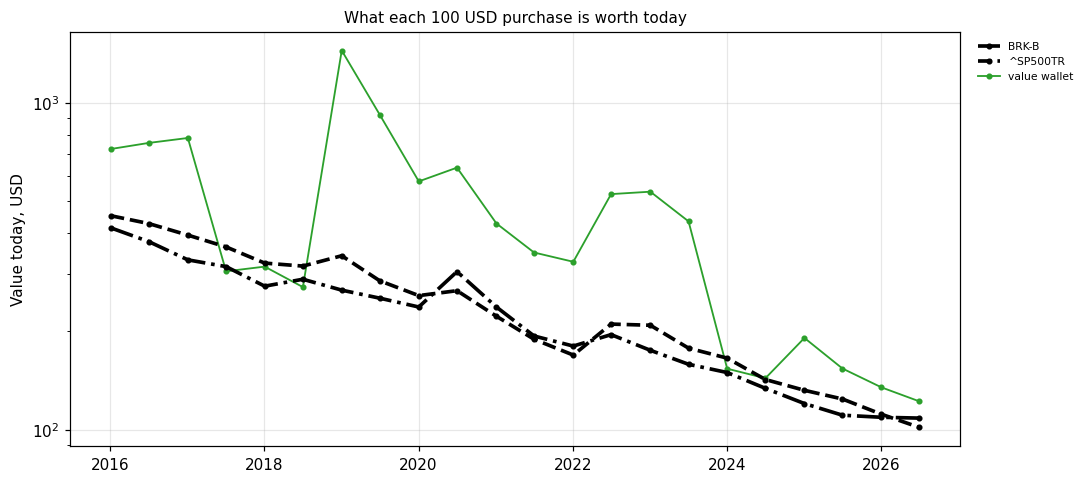
\includegraphics[width=1\textwidth]{yearly.png}
\caption{What each purchase is worth today, by date of purchase, on a logarithmic scale.}
\label{fig:yearly}
\end{figure}
\section{Value over time}
\begin{table}[H]
\centering
\small
\caption{Money put in and value today per start year (USD), and the money-weighted return a year.}\label{tab:value}
\begin{tabular}{l l r r r r}
\hline
Start & Holder & Put in & Value & Multiple & A year \\
\hline
2016 & Value wallet & 2,200 & 10,232 & 4.65 & 25.9\% \\
 & Value wallet with sells & 2,200 & 11,062 & 5.03 & 27.2\% \\
 & S\&P 500 & 2,200 & 5,383 & 2.45 & 15.3\% \\
 & Berkshire Hathaway & 2,200 & 4,938 & 2.24 & 13.9\% \\
\hline
2020 & Value wallet & 1,400 & 4,708 & 3.36 & 33.9\% \\
 & Value wallet with sells & 1,400 & 4,691 & 3.35 & 33.8\% \\
 & S\&P 500 & 1,400 & 2,480 & 1.77 & 15.9\% \\
 & Berkshire Hathaway & 1,400 & 2,415 & 1.73 & 15.2\% \\
\hline
2023 & Value wallet & 800 & 1,869 & 2.34 & 44.3\% \\
 & Value wallet with sells & 800 & 1,866 & 2.33 & 44.3\% \\
 & S\&P 500 & 800 & 1,164 & 1.46 & 18.7\% \\
 & Berkshire Hathaway & 800 & 1,066 & 1.33 & 14.2\% \\
\hline
2025 & Value wallet & 400 & 602 & 1.50 & 43.4\% \\
 & Value wallet with sells & 400 & 602 & 1.50 & 43.4\% \\
 & S\&P 500 & 400 & 469 & 1.17 & 15.7\% \\
 & Berkshire Hathaway & 400 & 449 & 1.12 & 11.1\% \\
\hline
\end{tabular}
\end{table}
Table \ref{tab:value} and Figure \ref{fig:value} follow the three investors. Each puts in 100 USD every January and July from the start year; the value wallet never sells. The return a year is money-weighted: the constant yearly rate that turns the payments into today's value.

The investor who started in 2016 earns 25.9\% a year against 15.3\% in the S\&P 500 and 13.9\% in Berkshire Hathaway. From 2020 the rates are 33.9\%, 15.9\% and 15.2\%; from 2025, over less than two years, 43.4\%, 15.7\% and 11.1\%. The wallet's value swings more than either comparison, because five companies of a few industries are far less diversified than the index or Berkshire.

The value wallet with sells buys the same picks with the same money, but at each decision it also sells part of any holding whose score has fallen; Section \ref{sec:selling} describes the rule. From 2016 it is worth 11,062 USD (27.2\% a year), from 2020 4,691 USD (33.8\%) and from 2025 602 USD (43.4\%).

\begin{figure}[H]
\centering
\begin{subfigure}[t]{0.480\textwidth}
\centering
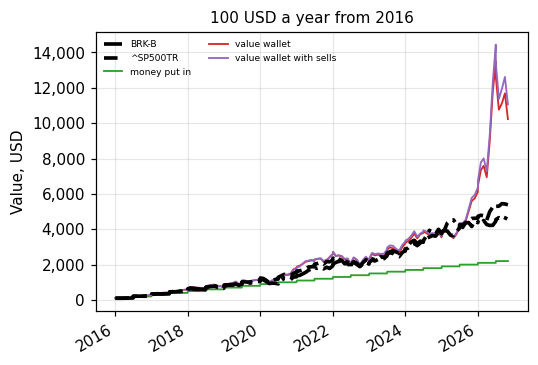
\includegraphics[width=\linewidth]{value_2016.png}
\caption{From 2016}
\end{subfigure}\hfill
\begin{subfigure}[t]{0.480\textwidth}
\centering
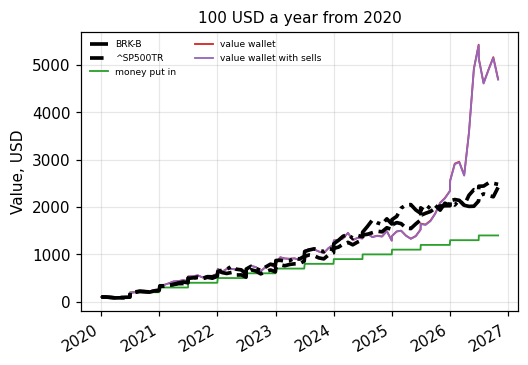
\includegraphics[width=\linewidth]{value_2020.png}
\caption{From 2020}
\end{subfigure}\hfill
\par\medskip
\begin{subfigure}[t]{0.480\textwidth}
\centering
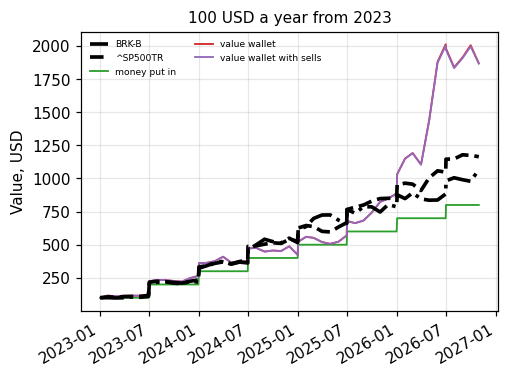
\includegraphics[width=\linewidth]{value_2023.png}
\caption{From 2023}
\end{subfigure}\hfill
\begin{subfigure}[t]{0.480\textwidth}
\centering
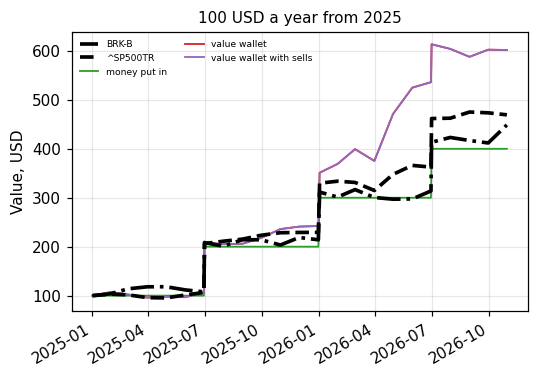
\includegraphics[width=\linewidth]{value_2025.png}
\caption{From 2025}
\end{subfigure}\hfill
\caption{Value of 100 USD every January and July from each start year, in USD, next to the money put in; the S\&P 500 dashed and Berkshire Hathaway dash-dot.}
\label{fig:value}
\end{figure}
\section{Selling below the threshold}
\label{sec:selling}
\begin{table}[H]
\centering
\small
\caption{Sales of the investor who started in 2020: share of each holding sold, its score on the 0-to-1 scale, and the proceeds.}\label{tab:sales}
\begin{tabular}{l p{11cm} r}
\hline
Year & Sold: share of the holding (score) & Proceeds, USD \\
\hline
2023-07 & HAS 9\% (score 0.36) & 3.34 \\
2024-01 & HAS 0\% (score 0.40) & 0.06 \\
2024-07 & HAS 58\% (score 0.17) & 17.54 \\
2025-01 & HAS 58\% (score 0.17) & 7.34 \\
2025-07 & HAS 14\% (score 0.34), INTC 8\% (score 0.37) & 4.68 \\
2026-01 & HAS 13\% (score 0.35), INTC 9\% (score 0.36) & 8.00 \\
2026-07 & HAS 38\% (score 0.25) & 2.34 \\
\hline
\end{tabular}
\end{table}
Each January and July, before buying, the wallet with sells checks every company it holds. The score is put on a scale from 0 to 1, the share of the most the company could score on the rules it is measured on. A holding scoring 0.4 or less is sold in part: the share sold is (0.4 less the score) divided by 0.4, so all of it at a score of 0 and almost none just under 0.4. Holdings are sold, never sold short. The proceeds are added to the decision's 100 USD and buy its picks. Table \ref{tab:sales} lists the 9 sales of the investor who started in 2020, worth 43 USD in all.

\section{Wallet contents}
Figure \ref{fig:contents} follows every company in the wallet with sells of the investor who started in 2020, month by month. A line starts or steps up when the company is bought, steps down when part of it is sold, and rises or falls with the price in between. The dashed lines follow the same money in the S\&P 500 and in Berkshire Hathaway, divided by the number of companies the wallet holds on the date, so they show what one holding would be worth in the index or in Berkshire. Appendix \ref{app:contents} gives each holding's value after every January's trades, the money put in and the proceeds of sales.

\begin{figure}[H]
\centering
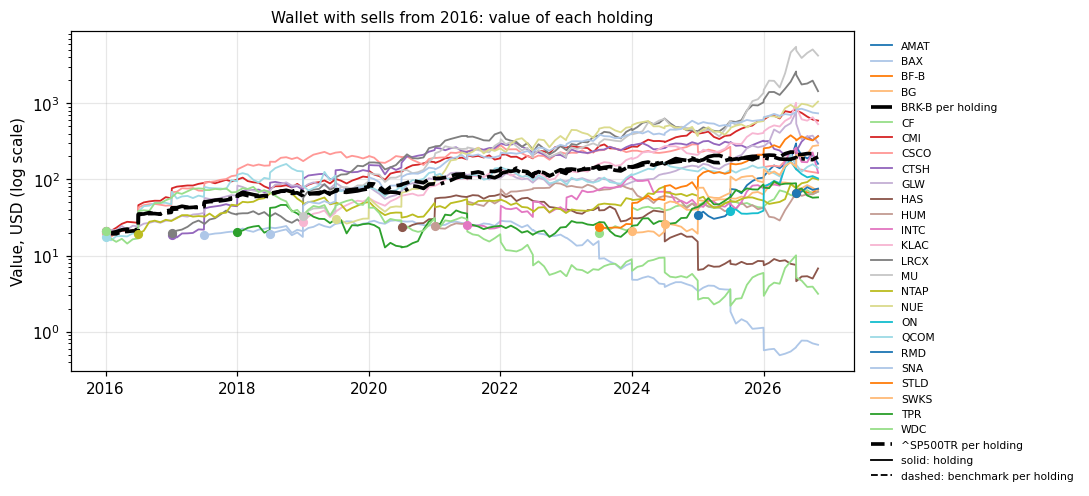
\includegraphics[width=1\textwidth]{contents.png}
\caption{Value of each holding in the wallet with sells (solid) and of the S\&P 500 and Berkshire Hathaway divided by the number of holdings (dashed), in USD on a logarithmic scale.}
\label{fig:contents}
\end{figure}
\section{Rules behind the winners}
\begin{table}[H]
\centering
\small
\caption{Dollars ahead of the same money in the S\&P 500, per pick: total, average and median of the picks that beat the index and of those that lagged it.}\label{tab:dollars}
\begin{tabular}{l r r r r}
\hline
Picks & Number & USD ahead, total & Average & Median \\
\hline
Beat the S\&P 500 & 63 & +5,495 & +87.2 & +16.8 \\
Lagged the S\&P 500 & 47 & -646 & -13.8 & -8.1 \\
\hline
All picks & 110 & +4,848 & +44.1 & +4.0 \\
\hline
\end{tabular}
\end{table}
Of the picks, 63 have done better than the S\&P 500 since their purchase and 47 have not, but a count treats a large win and a small loss alike. Table \ref{tab:dollars} weighs them in dollars: each pick's value today less what the same money would be worth in the S\&P 500. The winners are 5,495 USD ahead of the index and the laggards 646 USD behind, a net 4,848 USD, the wallet's whole lead over the index. The median winner is 17 USD ahead and the median laggard 8 USD behind; the average win is 6.3 times the average loss. The wins are concentrated: the 5 largest, MU Jan 2019, LRCX Jan 2017, MU Jul 2019, MU Jan 2023 and LRCX Jan 2019, make up 37\% of the winners' total.

Figure \ref{fig:rules} compares the mean points per rule of the winners and of the laggards on the day they were picked, each pick weighted by its dollars ahead or behind the index, so the large wins and losses count most; the rules are ordered by how much more the winners scored. The winners scored most above the others on price to tangible assets (E6), P/E (G6), P/E times P/B (G7) and 4-year earnings growth (E5); the picks that lagged scored higher on 10 years of profit (G3) and return on equity (B1). With so few picks, these differences describe this sample; they do not establish which rules work. Appendix \ref{app:rules} explains each rule, and Appendix \ref{app:weighting} tests whether the rule weights favour the rules that told winners from losers.

\begin{figure}[H]
\centering
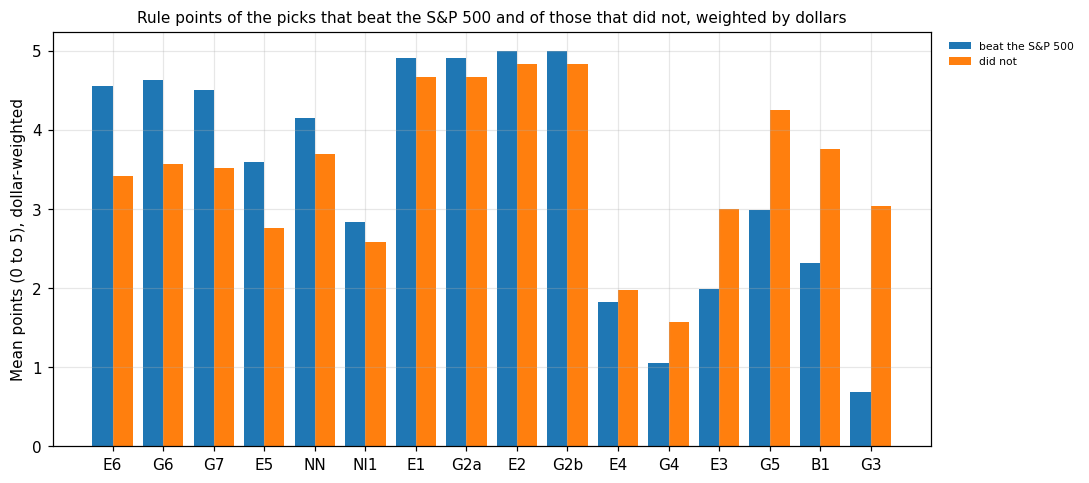
\includegraphics[width=1\textwidth]{rules.png}
\caption{Mean points per rule (0 to 5) of the picks that beat the S\&P 500 since purchase and of those that did not, each pick weighted by its dollars ahead or behind the index.}
\label{fig:rules}
\end{figure}
\section{The Magnificent 7}
\begin{table}[H]
\centering
\small
\caption{The Magnificent 7 on the score: score and score on the 0-to-1 scale on the latest score date, rank among the companies scored then, and median rank on the dates of the decisions since 2016.}\label{tab:peers}
\begin{tabular}{l r r r r}
\hline
Company & Score & Score 0 to 1 & Rank today & Median rank \\
\hline
Nvidia (NVDA) & 29.6 & 0.59 & 21 of 387 & 40 \\
Microsoft (MSFT) & 28.0 & 0.56 & 36 of 387 & 34 \\
Meta Platforms (META) & 25.7 & 0.73 & 55 of 387 & 199 \\
Alphabet Inc. (Class A) (GOOGL) & 24.7 & 0.56 & 68 of 387 & 30 \\
Tesla, Inc. (TSLA) & 18.6 & 0.38 & 160 of 387 & 156 \\
Amazon (AMZN) & 16.3 & 0.33 & 220 of 387 & 244 \\
Apple Inc. (AAPL) & 13.1 & 0.29 & 298 of 387 & 149 \\
\hline
\end{tabular}
\end{table}
The best-known growth companies of the period, the Magnificent 7, are rarely picked. On the latest score date Nvidia (NVDA) ranks highest of them, 21 of 387 companies, and Apple Inc. (AAPL) lowest at 298 (Table \ref{tab:peers}). The rules are Graham's and Buffett's, written to avoid paying a high price for growth: Figure \ref{fig:peers} shows that the Magnificent 7 score far fewer points than the picks on P/E times P/B (G7), P/E (G6), price to tangible assets (E6) and current dividend (E4), and more only on net income growth (NI1), 4-year earnings growth (E5) and 10-year earnings growth (G5).

The same 100 USD at each decision, split equally over the Magnificent 7 in the index on the date and never sold, is worth 22,613 USD from 2016 (39.0\% a year), 4,445 USD from 2020 (32.3\%) and 462 USD from 2025 (14.1\%), against 10,232, 4,708 and 602 USD in the value wallet. The comparison picks the Magnificent 7 with hindsight: they are named for having been the winners of these years.

\begin{figure}[H]
\centering
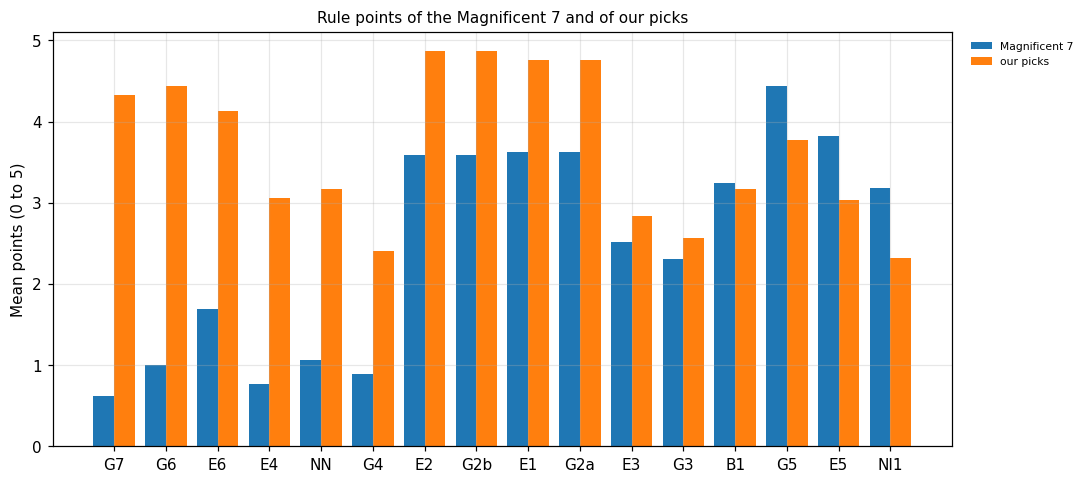
\includegraphics[width=1\textwidth]{peers.png}
\caption{Mean points per rule (0 to 5) of the Magnificent 7 and of our picks on the decision dates since 2016, the rules ordered by how many more points the picks scored.}
\label{fig:peers}
\end{figure}
\section{The next picks}
\begin{table}[H]
\centering
\small
\caption{The next picks on the latest score date: score, score on the 0-to-1 scale, weight and USD of each 100 USD.}\label{tab:next}
\begin{tabular}{l l r r r r}
\hline
Company & Sector & Score & Score 0 to 1 & Weight & USD \\
\hline
First Solar (FSLR) & Technology & 39.2 & 0.78 & 20.3\% & 20.28 \\
Cognizant (CTSH) & Technology & 38.9 & 0.78 & 20.1\% & 20.12 \\
Snap-on (SNA) & Industrials & 38.7 & 0.85 & 20.0\% & 20.03 \\
Skyworks Solutions (SWKS) & Technology & 38.5 & 0.77 & 19.9\% & 19.94 \\
ResMed (RMD) & Health care & 38.0 & 0.76 & 19.6\% & 19.64 \\
\hline
\end{tabular}
\end{table}
On the latest score date, 18 September 2026, the five highest-scoring companies are First Solar (FSLR), Cognizant (CTSH), Snap-on (SNA), Skyworks Solutions (SWKS) and ResMed (RMD) (Table \ref{tab:next}). Each would receive its share of the next decision's 100 USD and of any proceeds from sales. The decision is taken on the first trading day of January with the scores known then, which include the annual reports filed until that day; these picks are a preview and may change.

\subsection{Sell check}
\begin{table}[H]
\centering
\small
\caption{Holdings the rule would sell in part: value today, score on the 0-to-1 scale, share to sell and amount.}\label{tab:sell}
\begin{tabular}{l r r r r}
\hline
Company & Holding, USD & Score 0 to 1 & Sell & Sell, USD \\
\hline
Intel (INTC) & 115.97 & 0.40 & 1\% & 0.98 \\
Hasbro (HAS) & 5.59 & 0.25 & 38\% & 2.12 \\
\hline
\end{tabular}
\end{table}
The investor who started in 2020 holds 16 companies. With the scores of 18 September 2026, the rule would sell part of Intel (INTC), 1\% and Hasbro (HAS), 38\%, and keep the other 14 as they are (Table \ref{tab:sell}).

\section{Conclusions}
Bought twice a year and held, the value picks are worth more today than the same money in the S\&P 500 or in Berkshire Hathaway, for each of the three start years. The lead is uneven: the 8 purchases of Micron Technology (MU) make up 49\% of the 2020 investor's value, and the purchases of July 2017, January 2018, July 2018 and January 2024 trail the index.

Before the strategy is used, three steps are needed: the companies that left the index must be added to the data, the score must be tested on more decisions (each quarter instead of each year), and trading costs and taxes must be included.

\newpage
\appendix
\section{Every purchase}
\label{app:purchases}
{\small
\begin{longtable}{l l l r r r r r r r}
\caption{Every purchase of the wallet with sells of the investor who started in 2020: weight in the decision's purchase, USD invested (the decision's 100 USD and the proceeds of sales), split-adjusted price at purchase and today, USD sold from it later, USD it keeps today and its total return with dividends, (sold + kept) / invested - 1.}\label{tab:purchases}\\
\hline
Year & Company & Sector & Weight & In & Bought at & Now & Sold & Kept & Return \\
\hline
\endhead
2020-01 & NUE & Materials & 21\% & 21 & 55.12 & 273.87 &  & 120 & +463\% \\
2020-01 & CTSH & Technology & 21\% & 21 & 61.92 & 65.11 &  & 25 & +17\% \\
2020-01 & SNA & Industrials & 20\% & 20 & 169.00 & 355.66 &  & 50 & +151\% \\
2020-01 & MU & Technology & 20\% & 20 & 55.39 & 884.74 &  & 322 & +1538\% \\
2020-01 & CMI & Industrials & 18\% & 18 & 179.32 & 500.09 &  & 59 & +227\% \\
2020-07 & CTSH & Technology & 21\% & 21 & 56.42 & 65.11 &  & 27 & +28\% \\
2020-07 & NUE & Materials & 21\% & 21 & 40.38 & 273.87 &  & 157 & +652\% \\
2020-07 & HAS & Discretionary & 20\% & 20 & 74.69 & 119.09 & 18 & 3 & +3\% \\
2020-07 & MU & Technology & 19\% & 19 & 49.70 & 884.74 &  & 352 & +1726\% \\
2020-07 & SNA & Industrials & 19\% & 19 & 134.12 & 355.66 &  & 58 & +212\% \\
2021-01 & NUE & Materials & 21\% & 21 & 52.51 & 273.87 &  & 121 & +468\% \\
2021-01 & HAS & Discretionary & 21\% & 21 & 91.96 & 119.09 & 15 & 3 & -18\% \\
2021-01 & CTSH & Technology & 20\% & 20 & 79.42 & 65.11 &  & 18 & -10\% \\
2021-01 & MU & Technology & 19\% & 19 & 74.05 & 884.74 &  & 235 & +1125\% \\
2021-01 & HUM & Health care & 19\% & 19 & 412.19 & 414.50 &  & 20 & +6\% \\
2021-07 & SNA & Industrials & 21\% & 21 & 223.42 & 355.66 &  & 38 & +83\% \\
2021-07 & INTC & Technology & 20\% & 20 & 56.01 & 65.76 & 2 & 22 & +18\% \\
2021-07 & CMI & Industrials & 20\% & 20 & 242.13 & 500.09 &  & 47 & +133\% \\
2021-07 & HUM & Health care & 20\% & 20 & 447.63 & 414.50 &  & 19 & -2\% \\
2021-07 & MU & Technology & 19\% & 19 & 80.11 & 884.74 &  & 219 & +1033\% \\
2022-01 & SNA & Industrials & 20\% & 20 & 213.32 & 355.66 &  & 39 & +89\% \\
2022-01 & MU & Technology & 20\% & 20 & 95.75 & 884.74 &  & 193 & +845\% \\
2022-01 & CMI & Industrials & 20\% & 20 & 219.53 & 500.09 &  & 50 & +154\% \\
2022-01 & HUM & Health care & 20\% & 20 & 465.45 & 414.50 &  & 18 & -6\% \\
2022-01 & INTC & Technology & 20\% & 20 & 53.21 & 65.76 & 2 & 22 & +22\% \\
2022-07 & NUE & Materials & 22\% & 22 & 105.64 & 273.87 &  & 60 & +175\% \\
2022-07 & SNA & Industrials & 20\% & 20 & 198.24 & 355.66 &  & 40 & +101\% \\
2022-07 & MU & Technology & 20\% & 20 & 53.65 & 884.74 &  & 335 & +1585\% \\
2022-07 & INTC & Technology & 19\% & 19 & 36.34 & 65.76 & 3 & 31 & +76\% \\
2022-07 & CMI & Industrials & 19\% & 19 & 194.11 & 500.09 &  & 54 & +183\% \\
2023-01 & MU & Technology & 22\% & 22 & 50.37 & 884.74 &  & 384 & +1683\% \\
2023-01 & NUE & Materials & 21\% & 21 & 131.06 & 273.87 &  & 46 & +120\% \\
2023-01 & INTC & Technology & 19\% & 19 & 26.73 & 65.76 & 4 & 41 & +134\% \\
2023-01 & CTSH & Technology & 19\% & 19 & 57.59 & 65.11 &  & 23 & +21\% \\
2023-01 & SNA & Industrials & 19\% & 19 & 229.38 & 355.66 &  & 33 & +71\% \\
2023-07 & STLD & Materials & 22\% & 23 & 110.78 & 250.80 &  & 53 & +137\% \\
2023-07 & NUE & Materials & 21\% & 21 & 165.61 & 273.87 &  & 37 & +73\% \\
2023-07 & MU & Technology & 20\% & 21 & 63.90 & 884.74 &  & 297 & +1303\% \\
2023-07 & SNA & Industrials & 19\% & 20 & 286.86 & 355.66 &  & 27 & +35\% \\
2023-07 & CF & Materials & 18\% & 19 & 70.43 & 123.30 &  & 35 & +88\% \\
2024-01 & STLD & Materials & 22\% & 22 & 118.91 & 250.80 &  & 47 & +119\% \\
2024-01 & NUE & Materials & 21\% & 21 & 175.43 & 273.87 &  & 34 & +62\% \\
2024-01 & SWKS & Technology & 20\% & 20 & 109.11 & 87.58 &  & 17 & -12\% \\
2024-01 & SNA & Industrials & 19\% & 19 & 288.74 & 355.66 &  & 26 & +32\% \\
2024-01 & CF & Materials & 18\% & 18 & 81.61 & 123.30 &  & 30 & +61\% \\
2024-07 & NUE & Materials & 22\% & 25 & 157.00 & 273.87 &  & 46 & +80\% \\
2024-07 & STLD & Materials & 20\% & 24 & 129.15 & 250.80 &  & 47 & +100\% \\
2024-07 & SWKS & Technology & 20\% & 23 & 106.40 & 87.58 &  & 21 & -11\% \\
2024-07 & SNA & Industrials & 20\% & 23 & 256.90 & 355.66 &  & 34 & +47\% \\
2024-07 & BG & Staples & 19\% & 22 & 107.32 & 96.64 &  & 21 & -4\% \\
2025-01 & NUE & Materials & 21\% & 23 & 114.48 & 273.87 &  & 57 & +145\% \\
2025-01 & SWKS & Technology & 21\% & 22 & 88.45 & 87.58 &  & 23 & +5\% \\
2025-01 & STLD & Materials & 20\% & 22 & 111.93 & 250.80 &  & 49 & +129\% \\
2025-01 & AMAT & Technology & 19\% & 20 & 163.87 & 390.09 &  & 49 & +141\% \\
2025-01 & BG & Staples & 19\% & 20 & 77.57 & 96.64 &  & 27 & +31\% \\
2025-07 & SWKS & Technology & 21\% & 22 & 77.16 & 87.58 &  & 27 & +18\% \\
2025-07 & ON & Technology & 20\% & 21 & 53.60 & 71.67 &  & 29 & +34\% \\
2025-07 & SNA & Industrials & 20\% & 21 & 317.86 & 355.66 &  & 24 & +16\% \\
2025-07 & AMAT & Technology & 19\% & 20 & 183.76 & 390.09 &  & 44 & +114\% \\
2025-07 & STLD & Materials & 19\% & 20 & 130.16 & 250.80 &  & 38 & +95\% \\
2026-01 & SWKS & Technology & 21\% & 23 & 64.40 & 87.58 &  & 32 & +39\% \\
2026-01 & ON & Technology & 20\% & 22 & 56.70 & 71.67 &  & 28 & +26\% \\
2026-01 & SNA & Industrials & 20\% & 22 & 350.95 & 355.66 &  & 22 & +3\% \\
2026-01 & NUE & Materials & 20\% & 21 & 169.40 & 273.87 &  & 34 & +63\% \\
2026-01 & STLD & Materials & 19\% & 20 & 176.06 & 250.80 &  & 29 & +44\% \\
2026-07 & CTSH & Technology & 21\% & 21 & 41.07 & 65.11 &  & 34 & +59\% \\
2026-07 & SWKS & Technology & 20\% & 21 & 65.93 & 87.58 &  & 28 & +33\% \\
2026-07 & SNA & Industrials & 20\% & 20 & 403.28 & 355.66 &  & 18 & -11\% \\
2026-07 & RMD & Health care & 19\% & 20 & 201.10 & 229.94 &  & 23 & +15\% \\
2026-07 & BF-B & Staples & 19\% & 20 & 25.83 & 28.71 &  & 22 & +12\% \\
\hline
\end{longtable}}
\section{Wallet contents by year}
\label{app:contents}
\begin{table}[H]
\centering
\small
\caption{Wallet with sells of the investor who started in 2020: value of each holding after each January's trades and today (USD), and the money put in and the proceeds of sales to date, July decisions included.}\label{tab:contents}
\begin{tabular}{l r r r r r r r r }
\hline
Holding & 2020 & 2021 & 2022 & 2023 & 2024 & 2025 & 2026 & Now \\
\hline
CMI & 18 & 23 & 62 & 93 & 96 & 142 & 217 & 210 \\
CTSH & 21 & 77 & 87 & 76 & 100 & 105 & 113 & 126 \\
MU & 20 & 74 & 140 & 114 & 216 & 230 & 833 & 2,337 \\
NUE & 21 & 70 & 153 & 229 & 354 & 276 & 436 & 711 \\
SNA & 20 & 44 & 98 & 151 & 234 & 309 & 378 & 408 \\
HAS &  & 46 & 53 & 33 & 26 & 5 & 6 & 6 \\
HUM &  & 19 & 62 & 67 & 63 & 34 & 37 & 58 \\
INTC &  &  & 39 & 54 & 99 & 43 & 69 & 116 \\
CF &  &  &  &  & 40 & 43 & 41 & 65 \\
STLD &  &  &  &  & 46 & 86 & 184 & 265 \\
SWKS &  &  &  &  & 20 & 58 & 86 & 147 \\
BG &  &  &  &  &  & 37 & 45 & 48 \\
AMAT &  &  &  &  &  & 20 & 64 & 93 \\
ON &  &  &  &  &  &  & 45 & 57 \\
BF-B &  &  &  &  &  &  &  & 22 \\
RMD &  &  &  &  &  &  &  & 23 \\
\hline
Put in & 100 & 300 & 500 & 700 & 900 & 1,100 & 1,300 & 1,400 \\
Sold & 0 & 0 & 0 & 0 & 3 & 28 & 41 & 43 \\
Total & 100 & 353 & 694 & 818 & 1,294 & 1,388 & 2,554 & 4,691 \\
\hline
\end{tabular}
\end{table}
\section{Testing the weighting}
\label{app:weighting}
\begin{table}[H]
\centering
\small
\caption{Each rule's weight w\_r on the picks' dates (overall, for the picks that beat the S\&P 500 and for the others), the dollar-weighted mean points, the gap and the rank correlation with the return a year above the S\&P 500.}\label{tab:weighting}
\begin{tabular}{l r r r r r r r}
\hline
Rule & w\_r & w\_r beat & w\_r not & Pts beat & Pts not & Gap & Corr. \\
\hline
NN & 1.00 & 1.00 & 1.00 & 4.15 & 3.70 & +0.44 & -0.08 \\
E6 & 0.99 & 0.99 & 1.00 & 4.56 & 3.42 & +1.14 & +0.52 \\
G7 & 0.91 & 0.91 & 0.91 & 4.51 & 3.51 & +1.00 & +0.40 \\
G6 & 0.88 & 0.87 & 0.88 & 4.63 & 3.57 & +1.06 & +0.34 \\
G2b & 0.83 & 0.83 & 0.84 & 4.99 & 4.84 & +0.16 & +0.13 \\
E2 & 0.82 & 0.81 & 0.82 & 4.99 & 4.84 & +0.16 & +0.13 \\
B1 & 0.79 & 0.76 & 0.84 & 2.32 & 3.76 & -1.44 & -0.33 \\
G2a & 0.76 & 0.76 & 0.76 & 4.91 & 4.67 & +0.24 & +0.18 \\
E1 & 0.59 & 0.59 & 0.59 & 4.91 & 4.67 & +0.24 & +0.18 \\
G4 & 0.51 & 0.51 & 0.52 & 1.06 & 1.57 & -0.52 & -0.05 \\
NI1 & 0.39 & 0.38 & 0.39 & 2.84 & 2.59 & +0.25 & -0.13 \\
G3 & 0.27 & 0.26 & 0.28 & 0.69 & 3.03 & -2.34 & -0.31 \\
E5 & 0.25 & 0.25 & 0.25 & 3.60 & 2.77 & +0.83 & +0.26 \\
E3 & 0.20 & 0.20 & 0.21 & 1.99 & 3.00 & -1.01 & -0.29 \\
E4 & 0.19 & 0.19 & 0.19 & 1.83 & 1.98 & -0.15 & -0.09 \\
G5 & 0.18 & 0.18 & 0.19 & 2.99 & 4.25 & -1.27 & +0.01 \\
\hline
\end{tabular}
\end{table}
Each rule's points are multiplied by its weight, one less the share of companies passing it on the date, so a rule few companies pass counts more. A good weighting gives most weight to the rules whose points went with better returns. Table \ref{tab:weighting} sets each rule's mean weight on the dates the picks were made against two measures of how well it told the 110 picks apart: the gap between the mean points of the picks that beat the S\&P 500 and of those that did not, weighted by dollars as in Figure \ref{fig:rules}, and the rank correlation of the rule's points with each pick's return a year above the S\&P 500. Figure \ref{fig:weighting} plots weight against gap; a good weighting puts its rules on a rising line, with the heavy rules above zero.

Across the rules, the rank correlation of weight and gap is +0.61, and of weight and correlation +0.47.

The weighting leans towards the rules that worked, though far from fully. Weighted heavily but with a negative gap: return on equity (B1). A positive gap but a light weight: current ratio (lenient) (E1), 4-year earnings growth (E5) and net income growth (NI1). A rule's weight hardly differs between the dates of winning and losing picks (columns w\_r beat and w\_r not), because it is set across all companies on a date, not per pick. These differences suggest where the weighting could be tuned; any change must be tested on years it was not fitted on.

\begin{figure}[H]
\centering
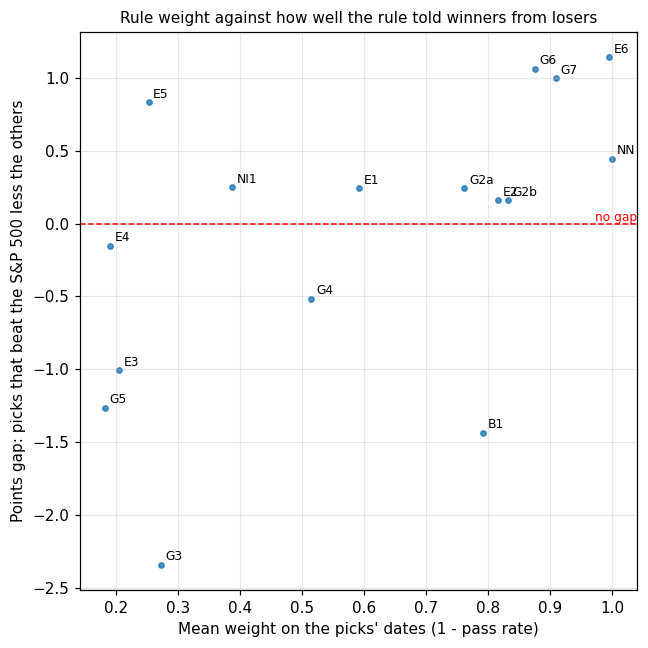
\includegraphics[width=0.6\textwidth]{weighting.png}
\caption{Each rule's mean weight against the gap in points between the picks that beat the S\&P 500 and the others, weighted by dollars; rules above the line told winners from losers.}
\label{fig:weighting}
\end{figure}
\section{Forward information}
\label{app:lookahead}
\begin{table}[H]
\centering
\small
\caption{Truncation check: companies scored on the date, companies whose score differs when every input is cut at the date (per score), and whether the five picks are the same.}\label{tab:lookahead}
\begin{tabular}{l r r r r r l}
\hline
Date & Companies & Score & Score 0 to 1 & Unweighted & Share passed & Same picks \\
\hline
2018-12-21 & 296 & 2 & 2 & 2 & 0 & yes \\
2022-12-16 & 339 & 274 & 329 & 3 & 1 & yes \\
2025-12-19 & 376 & 0 & 0 & 0 & 0 & yes \\
\hline
\end{tabular}
\end{table}
A score must use only what was known on its date. Four guards are built in. A company's figures count from the day its annual report was filed with the SEC, and of all the figures filed for a year only the first reported is used, never a later restatement. Prices are the close on the scoring date and dividends are counted by their ex-date. Each January and July purchase uses the scores of the rebalance date two weeks before it. Rule weights come from the companies on the date alone.

These guards are tested by cutting every input at a date as if it were that day (filings filed on or before it, prices and dividends up to it), scoring the companies again and comparing the scores with the full run (Table \ref{tab:lookahead}). Any difference means information from after the date reached a score. On 21 December 2018, 16 December 2022 and 19 December 2025 the picks were the same. The scores were identical on 19 December 2025; on the other dates a few companies differ by about one point, because when a company reports an item under two labels, the label is chosen by the company's later use. The fix, choosing the label from filings known on the date, is pending; the check runs as a unit test and will pass once it is in.

Three sources of forward information are outside this test. Only today's S\&P 500 members are scored: companies join the universe only from the date they entered the index, but companies that later left it are missing, which flatters every result. Sectors are today's, used to leave out Financials and Real Estate in earlier years. And the score's design was settled while looking at 2016 to 2026, so only the years from 2022 test it fairly.

\subsection{Companies missing from the data}
\begin{table}[H]
\centering
\small
\caption{Companies that left the S\&P 500 since each start year, all missing from the data: in all, on their market value, and through an acquisition or another reason.}\label{tab:survivors}
\begin{tabular}{l r r r}
\hline
Start & Left the index & On market value & Acquired or other \\
\hline
2016 & 230 & 97 & 133 \\
2020 & 125 & 75 & 50 \\
2023 & 69 & 47 & 22 \\
2025 & 37 & 24 & 13 \\
\hline
\end{tabular}
\end{table}
Table \ref{tab:survivors} counts the companies that left the S\&P 500 after each start year; none of them is in the data, of any sector. Most left through an acquisition, often at a premium; those that dropped out on their market value are the likely losers a real investor could have picked. The later the start, the fewer are missing, which is why the investor who started in 2020 is the reference of this report. The bias is removed only when the historical members of the index are added to the data.

\section{The rules}
\label{app:rules}
\begin{table}[H]
\centering
\small
\caption{The rules: what each measures, the better direction and when a company passes.}\label{tab:rules}
\begin{tabular}{l p{2.2cm} p{5.2cm} l p{2.8cm}}
\hline
Rule & Name & What it measures & Better & Passes when \\
\hline
G2a & current ratio & Current assets divided by current liabilities: what the company owns against what it owes within a year. & higher & at least 2.0 \\
G2b & debt to working capital & Long-term debt divided by net current assets (current assets less current liabilities). & lower & at most 1.0 \\
G3 & 10 years of profit & Number of the last 10 fiscal years with positive earnings per share. & higher & all 10 years \\
G4 & 20 years of dividends & Number of the 20 calendar years before the decision in which a dividend was paid. & higher & all 20 years \\
G5 & 10-year earnings growth & Average earnings per share of the last 3 years over the average of 3 years a decade earlier. & higher & at least 1.33 \\
G6 & P/E & Price over the average earnings per share of the last 3 years. & lower & at most 15.0 \\
G7 & P/E times P/B & P/E as in G6 times the price over book value per share. & lower & P/B at most 1.5, or the product at most 22.5 \\
E1 & current ratio (lenient) & Current ratio, as G2a. & higher & at least 1.5 \\
E2 & debt to working capital (lenient) & Long-term debt over net current assets, as G2b. & lower & at most 1.1 \\
E3 & 5 years of profit & Number of the last 5 fiscal years with positive earnings per share. & higher & all 5 years \\
E4 & current dividend & Dividends paid over the last 365 days, as a yield on the price. & higher & any dividend \\
E5 & 4-year earnings growth & Change in earnings per share over 4 years, relative to the earlier figure. & higher & earnings per share grew \\
E6 & price to tangible assets & Market value over net tangible assets (equity less goodwill and other intangible assets). & lower & at most 1.2 \\
NN & net-net & Market value over net current asset value (current assets less all liabilities). & lower & at most 0.67 \\
B1 & return on equity & Number of the last 10 years with return on equity (net income over equity) of at least 15\%. & higher & at least 7 years, and long-term debt at most 0.5 times equity \\
NI1 & net income growth & Growth of net income from the year before to the latest year. & higher & net income grew \\
\hline
\end{tabular}
\end{table}
Table \ref{tab:rules} explains each rule: what it measures, whether a higher or a lower value earns more points, and when a company passes it. The points come from the company's rank on the measure among all companies on the date; the pass threshold sets the rule's weight. Rules G follow Graham's defensive investor (The Intelligent Investor, chapter 14), rules E his enterprising investor (chapter 15) and his net-net test (NN), B1 Buffett's return on equity, and NI1 was added for net income growth. Two pairs test the same measure at different strictness (G2a and E1, G2b and E2), so the current ratio and debt count twice.

\end{document}
